\section{Architecture}
The \confignoc{} incorporates a 2D mesh network for communication across all the routers and neuron cores.
An extra link is attached to the \confignoc{} that enables interfacing with the external world (shown as the red arrow in \cref{fig:config_noc_ext}).
Compared to the \eventnoc{}, intercommunication does not occur between neuron cores.

\begin{figure}[hbtp]
\centering    
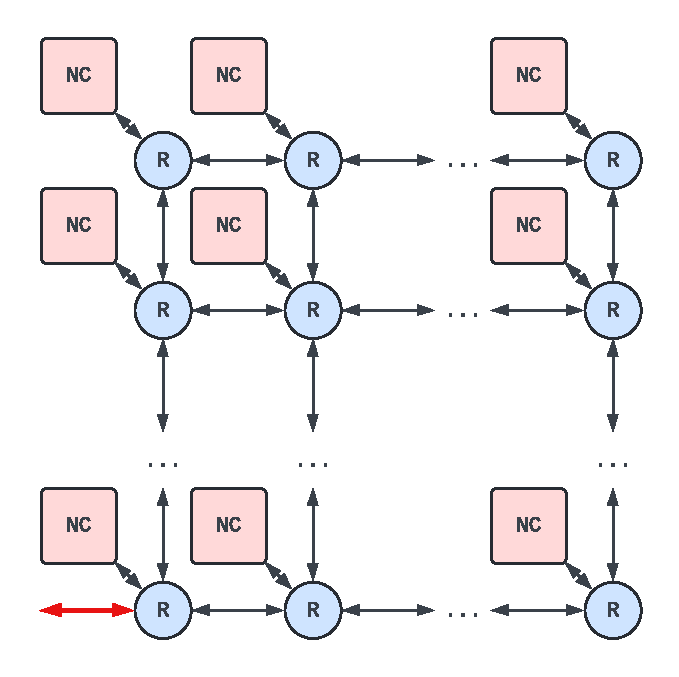
\includegraphics[width=0.45\textwidth]{assets/config_noc_inj.pdf}
\caption{\confignoc{} including the external inferface}
\label{fig:config_noc_ext}
\end{figure}

The communication links between nodes are 16-bits wide, determining the amount of data that can be transferred concurrently.
The \confignoc{} uses a packet-switched communication protocol, where data is transmitted in the form of independent packets routed through the network.

For routing, XY routing, a deterministic algorithm, is employed \autocite{glassTurnModelAdaptive1992}.
Packets first travel horizontally along the X-dimension until they reach the destination column, and then vertically along the Y-dimension to the destination row.

At each router, wormhole switching is utilized.
This is a low-latency technique where packets are divided into smaller units called flits.
A header flit establishes the path, and the remaining flits follow in a pipelined manner, minimizing delays as the packet ``burrows'' through the network.
Whenever the header has been processed, all the payload data will follow it and cannot be interrupted.
The flits in the \confignoc{} are of the same size as phits.
A phit is the amount of bits that can be transferred over a single hop in one clock cycle.

A key characteristic of the \confignoc{}'s architecture is its \SI{800}{MHz} clock frequency.
This clock governs the rate of data transmission across the network, influencing the overall performance of the on-chip communication.

% Unlike the \confignoc{}, the \eventnoc{} uses wraparound links that helps to drastically reduce the average amount of hops a packet has to take.
% Wraparound links do not provide any noticeable benefits to the \confignoc{} since these interactions do not occur with the \confignoc{}.
Most of the high traffic data transactions occur when data is written to the neuron cores' SRAMs.
This process only injects the data in the \confignoc{} via a single point.
